% 网络安全攻防竞赛实践课程笔记 —— 主文档（正文排版集中在 0.样式.tex，章节文件只放内容）
% 编译：xelatex 1.main.tex 两遍；成品输出见 build.ps1
\documentclass[11pt,a4paper,oneside]{article}
\usepackage[UTF8,fontset=windows,scheme=plain]{ctex}
\usepackage{fontspec}
\setmainfont{Times New Roman}
\setsansfont{Microsoft YaHei}

\newcommand{\YHBcourse}{网络安全攻防竞赛实践}
\newcommand{\YHBversion}{v1.1}
\newcommand{\YHBquote}{以攻防为刃，守护数字边界；以技术为基，探索安全世界。}
\newcommand{\YHBcoverSize}{33pt}
\newcommand{\YHBcoverLead}{40pt}
\usepackage{xcolor}
\definecolor{yhbAccent}{HTML}{262626}
\definecolor{yhbAccent2}{HTML}{8C3030}
% ============================================================
% 0.样式.tex —— 课程笔记统一正文排版
% 用法：主文件先定义课程信息与主色，再 % ============================================================
% 0.样式.tex —— 课程笔记统一正文排版
% 用法：主文件先定义课程信息与主色，再 % ============================================================
% 0.样式.tex —— 课程笔记统一正文排版
% 用法：主文件先定义课程信息与主色，再 \input{0.样式.tex}
%   \newcommand{\YHBcourse}{微积分A}      % 课程名（页眉与书签用）
%   \newcommand{\YHBversion}{v1.2}        % 版本号（封面用）
%   \newcommand{\YHBquote}{……}            % 封面题句
%   \definecolor{yhbAccent}{HTML}{24465C} % 主色（深）
%   \definecolor{yhbAccent2}{HTML}{347A80}% 辅色（浅）
%   \YHBbooktrue / \YHBbookfalse          % 是否 book 文档类（有 \chapter）
% 章节文件只写内容，不要重复 \usepackage、不要改字号。
% ============================================================

% ---------- 页面与字体 ----------
\usepackage{geometry}
\geometry{a4paper,left=24mm,right=24mm,top=23mm,bottom=24mm,headheight=15pt,headsep=7mm,footskip=13mm}
\usepackage{microtype}
\usepackage{amsmath,amssymb,amsfonts,mathtools}
\usepackage{esint}
\usepackage{graphicx}
\usepackage{adjustbox}
\usepackage{array,booktabs,multirow,makecell,tabularx,longtable}
\usepackage{xcolor,colortbl}
\usepackage{enumitem}
\usepackage{needspace,etoolbox}
\usepackage{titlesec,titletoc}
\usepackage{fancyhdr}
\usepackage{caption}
\usepackage[most]{tcolorbox}

% ---------- 颜色别名（章节里用的旧名继续有效） ----------
\colorlet{mainblue}{yhbAccent}
\colorlet{secondcyan}{yhbAccent2}
\colorlet{thirdteal}{yhbAccent2}
\colorlet{highlight}{yhbAccent!6!white}
\colorlet{tablehead}{yhbAccent!12!white}
\definecolor{textgray}{HTML}{4A5057}

% ---------- 课程标签 ----------
\providecommand{\YHBdoclabel}{课程笔记}
% ---------- 正文节奏 ----------
\linespread{1.3}
\setlength{\parindent}{0pt}
\setlength{\parskip}{6pt plus 1.5pt minus 1.5pt}
\setlength{\emergencystretch}{2.5em}
\raggedbottom
\widowpenalty=10000
\clubpenalty=10000
\setlength{\tabcolsep}{7pt}
\renewcommand{\arraystretch}{1.3}
\allowdisplaybreaks[2]
\AtBeginDocument{%
  \setlength{\abovedisplayskip}{10pt plus 2pt minus 2pt}%
  \setlength{\belowdisplayskip}{10pt plus 2pt minus 2pt}%
  \setlength{\abovedisplayshortskip}{6pt}%
  \setlength{\belowdisplayshortskip}{6pt}%
}
\captionsetup{font=small,labelfont=bf,skip=6pt}

% ---------- 列表 ----------
\setlist{leftmargin=2em,labelsep=0.6em,itemsep=4pt,parsep=2pt,topsep=6pt,partopsep=0pt}
\setlist[itemize,2]{label=\textbullet,leftmargin=1.6em}

% ---------- 标题层级 ----------
\ifdefined\YHBbooktrue
  \titleformat{\chapter}[display]
    {\sffamily\bfseries\color{yhbAccent}}
    {\normalsize\sffamily 第\,\thechapter\,章}
    {6pt}
    {\LARGE}
    [{\vspace{5pt}{\color{yhbAccent!55}\titlerule[1pt]}}]
  \titlespacing*{\chapter}{0pt}{14pt}{24pt}
  \titleformat{\section}{\Large\sffamily\bfseries\color{yhbAccent}}{\thesection}{0.7em}{}
  \titlespacing*{\section}{0pt}{18pt plus 3pt minus 2pt}{8pt}
\else
  \titleformat{\section}{\Large\sffamily\bfseries\color{yhbAccent}}{\thesection}{0.7em}{}[{\vspace{3pt}{\color{yhbAccent!45}\titlerule[0.7pt]}}]
  \titlespacing*{\section}{0pt}{18pt plus 3pt minus 2pt}{9pt}
\fi
\titleformat{\subsection}{\large\sffamily\bfseries\color{yhbAccent!85!black}}{\thesubsection}{0.7em}{}
\titleformat{\subsubsection}{\normalsize\bfseries\color{black!85}}{\thesubsubsection}{0.7em}{}
\titlespacing*{\subsection}{0pt}{12pt plus 2pt minus 1pt}{5pt}
\titlespacing*{\subsubsection}{0pt}{9pt plus 2pt minus 1pt}{4pt}
\pretocmd{\section}{\Needspace{6\baselineskip}}{}{}
\pretocmd{\subsection}{\Needspace{5\baselineskip}}{}{}
\pretocmd{\subsubsection}{\Needspace{4\baselineskip}}{}{}

\ifdefined\YHBbooktrue
  \setcounter{secnumdepth}{2}
  \setcounter{tocdepth}{1}
\else
  \setcounter{secnumdepth}{3}
  \setcounter{tocdepth}{2}
\fi
\renewcommand{\contentsname}{目录}
% 目录编号颜色由 titletoc 的 titlecontents 控制，不再重定义 \numberline

% ---------- 目录样式 ----------
\ifdefined\YHBbooktrue
  \titlecontents{chapter}[0pt]
    {\addvspace{6pt}\sffamily\bfseries\color{yhbAccent}}
    {\contentslabel{2.2em}}{}{\titlerule*[0.6em]{.}\contentspage}
  \titlecontents{section}[2.2em]
    {\addvspace{2pt}}
    {\contentslabel{2.2em}}{}{\titlerule*[0.6em]{.}\contentspage}
\else
  \titlecontents{section}[0pt]
    {\addvspace{5pt}\sffamily\bfseries\color{yhbAccent}}
    {\contentslabel{2.2em}}{}{\titlerule*[0.6em]{.}\contentspage}
  \titlecontents{subsection}[2.2em]
    {\addvspace{2pt}}
    {\contentslabel{2.4em}}{}{\titlerule*[0.6em]{.}\contentspage}
\fi

% ---------- 页眉页脚 ----------
\pagestyle{fancy}
\fancyhf{}
\fancyhead[L]{\footnotesize\sffamily\color{textgray}\YHBcourse\ \YHBdoclabel}
\ifdefined\YHBbooktrue
  \fancyhead[R]{\footnotesize\sffamily\color{textgray}\nouppercase{\leftmark}}
  \renewcommand{\chaptermark}[1]{\markboth{#1}{}}
\else
  \fancyhead[R]{\footnotesize\sffamily\color{textgray}\nouppercase{\rightmark}}
  \renewcommand{\sectionmark}[1]{\markright{#1}}
\fi
\fancyfoot[C]{\footnotesize\color{textgray}\thepage}
\renewcommand{\headrulewidth}{0.35pt}
\renewcommand{\headrule}{{\color{yhbAccent!45}\hrule width\headwidth height\headrulewidth}}
\fancypagestyle{plain}{%
  \fancyhf{}%
  \fancyfoot[C]{\footnotesize\color{textgray}\thepage}%
  \renewcommand{\headrulewidth}{0pt}%
}

% ---------- 公式与考点框 ----------
\newcommand{\keyformula}[1]{%
  \begin{tcolorbox}[enhanced,breakable,colback=highlight,colframe=yhbAccent!30!white,boxrule=0.5pt,arc=2.5pt,left=11pt,right=11pt,top=9pt,bottom=9pt,boxsep=0pt,before skip=11pt,after skip=11pt,halign=center,width=\linewidth]
  \adjustbox{max width=\linewidth-2em}{$\displaystyle #1$}
  \end{tcolorbox}}
\newcommand{\corepoint}[1]{%
  \begin{tcolorbox}[enhanced,breakable,colback=highlight,colframe=yhbAccent2,boxrule=0pt,borderline west={2.4pt}{0pt}{yhbAccent2},arc=0pt,left=11pt,right=11pt,top=8pt,bottom=8pt,before skip=11pt,after skip=11pt]
  \textbf{\color{yhbAccent}核心考点}\quad #1
  \end{tcolorbox}}
\newcommand{\symb}[2]{\textbf{#1}：#2\par}

% ---------- 超链接（务必最后加载） ----------
\usepackage[unicode=true,colorlinks=true,linkcolor=yhbAccent,citecolor=yhbAccent,urlcolor=yhbAccent!85!black,pdfborder={0 0 0},bookmarksnumbered=true,pdfstartview=FitH]{hyperref}
\usepackage{hypcap}
\hypersetup{pdftitle={\YHBcourse 课程笔记},pdfauthor={浮萍},pdfsubject={课程学习与复习笔记},pdfcreator={XeLaTeX}}

%   \newcommand{\YHBcourse}{微积分A}      % 课程名（页眉与书签用）
%   \newcommand{\YHBversion}{v1.2}        % 版本号（封面用）
%   \newcommand{\YHBquote}{……}            % 封面题句
%   \definecolor{yhbAccent}{HTML}{24465C} % 主色（深）
%   \definecolor{yhbAccent2}{HTML}{347A80}% 辅色（浅）
%   \YHBbooktrue / \YHBbookfalse          % 是否 book 文档类（有 \chapter）
% 章节文件只写内容，不要重复 \usepackage、不要改字号。
% ============================================================

% ---------- 页面与字体 ----------
\usepackage{geometry}
\geometry{a4paper,left=24mm,right=24mm,top=23mm,bottom=24mm,headheight=15pt,headsep=7mm,footskip=13mm}
\usepackage{microtype}
\usepackage{amsmath,amssymb,amsfonts,mathtools}
\usepackage{esint}
\usepackage{graphicx}
\usepackage{adjustbox}
\usepackage{array,booktabs,multirow,makecell,tabularx,longtable}
\usepackage{xcolor,colortbl}
\usepackage{enumitem}
\usepackage{needspace,etoolbox}
\usepackage{titlesec,titletoc}
\usepackage{fancyhdr}
\usepackage{caption}
\usepackage[most]{tcolorbox}

% ---------- 颜色别名（章节里用的旧名继续有效） ----------
\colorlet{mainblue}{yhbAccent}
\colorlet{secondcyan}{yhbAccent2}
\colorlet{thirdteal}{yhbAccent2}
\colorlet{highlight}{yhbAccent!6!white}
\colorlet{tablehead}{yhbAccent!12!white}
\definecolor{textgray}{HTML}{4A5057}

% ---------- 课程标签 ----------
\providecommand{\YHBdoclabel}{课程笔记}
% ---------- 正文节奏 ----------
\linespread{1.3}
\setlength{\parindent}{0pt}
\setlength{\parskip}{6pt plus 1.5pt minus 1.5pt}
\setlength{\emergencystretch}{2.5em}
\raggedbottom
\widowpenalty=10000
\clubpenalty=10000
\setlength{\tabcolsep}{7pt}
\renewcommand{\arraystretch}{1.3}
\allowdisplaybreaks[2]
\AtBeginDocument{%
  \setlength{\abovedisplayskip}{10pt plus 2pt minus 2pt}%
  \setlength{\belowdisplayskip}{10pt plus 2pt minus 2pt}%
  \setlength{\abovedisplayshortskip}{6pt}%
  \setlength{\belowdisplayshortskip}{6pt}%
}
\captionsetup{font=small,labelfont=bf,skip=6pt}

% ---------- 列表 ----------
\setlist{leftmargin=2em,labelsep=0.6em,itemsep=4pt,parsep=2pt,topsep=6pt,partopsep=0pt}
\setlist[itemize,2]{label=\textbullet,leftmargin=1.6em}

% ---------- 标题层级 ----------
\ifdefined\YHBbooktrue
  \titleformat{\chapter}[display]
    {\sffamily\bfseries\color{yhbAccent}}
    {\normalsize\sffamily 第\,\thechapter\,章}
    {6pt}
    {\LARGE}
    [{\vspace{5pt}{\color{yhbAccent!55}\titlerule[1pt]}}]
  \titlespacing*{\chapter}{0pt}{14pt}{24pt}
  \titleformat{\section}{\Large\sffamily\bfseries\color{yhbAccent}}{\thesection}{0.7em}{}
  \titlespacing*{\section}{0pt}{18pt plus 3pt minus 2pt}{8pt}
\else
  \titleformat{\section}{\Large\sffamily\bfseries\color{yhbAccent}}{\thesection}{0.7em}{}[{\vspace{3pt}{\color{yhbAccent!45}\titlerule[0.7pt]}}]
  \titlespacing*{\section}{0pt}{18pt plus 3pt minus 2pt}{9pt}
\fi
\titleformat{\subsection}{\large\sffamily\bfseries\color{yhbAccent!85!black}}{\thesubsection}{0.7em}{}
\titleformat{\subsubsection}{\normalsize\bfseries\color{black!85}}{\thesubsubsection}{0.7em}{}
\titlespacing*{\subsection}{0pt}{12pt plus 2pt minus 1pt}{5pt}
\titlespacing*{\subsubsection}{0pt}{9pt plus 2pt minus 1pt}{4pt}
\pretocmd{\section}{\Needspace{6\baselineskip}}{}{}
\pretocmd{\subsection}{\Needspace{5\baselineskip}}{}{}
\pretocmd{\subsubsection}{\Needspace{4\baselineskip}}{}{}

\ifdefined\YHBbooktrue
  \setcounter{secnumdepth}{2}
  \setcounter{tocdepth}{1}
\else
  \setcounter{secnumdepth}{3}
  \setcounter{tocdepth}{2}
\fi
\renewcommand{\contentsname}{目录}
% 目录编号颜色由 titletoc 的 titlecontents 控制，不再重定义 \numberline

% ---------- 目录样式 ----------
\ifdefined\YHBbooktrue
  \titlecontents{chapter}[0pt]
    {\addvspace{6pt}\sffamily\bfseries\color{yhbAccent}}
    {\contentslabel{2.2em}}{}{\titlerule*[0.6em]{.}\contentspage}
  \titlecontents{section}[2.2em]
    {\addvspace{2pt}}
    {\contentslabel{2.2em}}{}{\titlerule*[0.6em]{.}\contentspage}
\else
  \titlecontents{section}[0pt]
    {\addvspace{5pt}\sffamily\bfseries\color{yhbAccent}}
    {\contentslabel{2.2em}}{}{\titlerule*[0.6em]{.}\contentspage}
  \titlecontents{subsection}[2.2em]
    {\addvspace{2pt}}
    {\contentslabel{2.4em}}{}{\titlerule*[0.6em]{.}\contentspage}
\fi

% ---------- 页眉页脚 ----------
\pagestyle{fancy}
\fancyhf{}
\fancyhead[L]{\footnotesize\sffamily\color{textgray}\YHBcourse\ \YHBdoclabel}
\ifdefined\YHBbooktrue
  \fancyhead[R]{\footnotesize\sffamily\color{textgray}\nouppercase{\leftmark}}
  \renewcommand{\chaptermark}[1]{\markboth{#1}{}}
\else
  \fancyhead[R]{\footnotesize\sffamily\color{textgray}\nouppercase{\rightmark}}
  \renewcommand{\sectionmark}[1]{\markright{#1}}
\fi
\fancyfoot[C]{\footnotesize\color{textgray}\thepage}
\renewcommand{\headrulewidth}{0.35pt}
\renewcommand{\headrule}{{\color{yhbAccent!45}\hrule width\headwidth height\headrulewidth}}
\fancypagestyle{plain}{%
  \fancyhf{}%
  \fancyfoot[C]{\footnotesize\color{textgray}\thepage}%
  \renewcommand{\headrulewidth}{0pt}%
}

% ---------- 公式与考点框 ----------
\newcommand{\keyformula}[1]{%
  \begin{tcolorbox}[enhanced,breakable,colback=highlight,colframe=yhbAccent!30!white,boxrule=0.5pt,arc=2.5pt,left=11pt,right=11pt,top=9pt,bottom=9pt,boxsep=0pt,before skip=11pt,after skip=11pt,halign=center,width=\linewidth]
  \adjustbox{max width=\linewidth-2em}{$\displaystyle #1$}
  \end{tcolorbox}}
\newcommand{\corepoint}[1]{%
  \begin{tcolorbox}[enhanced,breakable,colback=highlight,colframe=yhbAccent2,boxrule=0pt,borderline west={2.4pt}{0pt}{yhbAccent2},arc=0pt,left=11pt,right=11pt,top=8pt,bottom=8pt,before skip=11pt,after skip=11pt]
  \textbf{\color{yhbAccent}核心考点}\quad #1
  \end{tcolorbox}}
\newcommand{\symb}[2]{\textbf{#1}：#2\par}

% ---------- 超链接（务必最后加载） ----------
\usepackage[unicode=true,colorlinks=true,linkcolor=yhbAccent,citecolor=yhbAccent,urlcolor=yhbAccent!85!black,pdfborder={0 0 0},bookmarksnumbered=true,pdfstartview=FitH]{hyperref}
\usepackage{hypcap}
\hypersetup{pdftitle={\YHBcourse 课程笔记},pdfauthor={浮萍},pdfsubject={课程学习与复习笔记},pdfcreator={XeLaTeX}}

%   \newcommand{\YHBcourse}{微积分A}      % 课程名（页眉与书签用）
%   \newcommand{\YHBversion}{v1.2}        % 版本号（封面用）
%   \newcommand{\YHBquote}{……}            % 封面题句
%   \definecolor{yhbAccent}{HTML}{24465C} % 主色（深）
%   \definecolor{yhbAccent2}{HTML}{347A80}% 辅色（浅）
%   \YHBbooktrue / \YHBbookfalse          % 是否 book 文档类（有 \chapter）
% 章节文件只写内容，不要重复 \usepackage、不要改字号。
% ============================================================

% ---------- 页面与字体 ----------
\usepackage{geometry}
\geometry{a4paper,left=24mm,right=24mm,top=23mm,bottom=24mm,headheight=15pt,headsep=7mm,footskip=13mm}
\usepackage{microtype}
\usepackage{amsmath,amssymb,amsfonts,mathtools}
\usepackage{esint}
\usepackage{graphicx}
\usepackage{adjustbox}
\usepackage{array,booktabs,multirow,makecell,tabularx,longtable}
\usepackage{xcolor,colortbl}
\usepackage{enumitem}
\usepackage{needspace,etoolbox}
\usepackage{titlesec,titletoc}
\usepackage{fancyhdr}
\usepackage{caption}
\usepackage[most]{tcolorbox}

% ---------- 颜色别名（章节里用的旧名继续有效） ----------
\colorlet{mainblue}{yhbAccent}
\colorlet{secondcyan}{yhbAccent2}
\colorlet{thirdteal}{yhbAccent2}
\colorlet{highlight}{yhbAccent!6!white}
\colorlet{tablehead}{yhbAccent!12!white}
\definecolor{textgray}{HTML}{4A5057}

% ---------- 课程标签 ----------
\providecommand{\YHBdoclabel}{课程笔记}
% ---------- 正文节奏 ----------
\linespread{1.3}
\setlength{\parindent}{0pt}
\setlength{\parskip}{6pt plus 1.5pt minus 1.5pt}
\setlength{\emergencystretch}{2.5em}
\raggedbottom
\widowpenalty=10000
\clubpenalty=10000
\setlength{\tabcolsep}{7pt}
\renewcommand{\arraystretch}{1.3}
\allowdisplaybreaks[2]
\AtBeginDocument{%
  \setlength{\abovedisplayskip}{10pt plus 2pt minus 2pt}%
  \setlength{\belowdisplayskip}{10pt plus 2pt minus 2pt}%
  \setlength{\abovedisplayshortskip}{6pt}%
  \setlength{\belowdisplayshortskip}{6pt}%
}
\captionsetup{font=small,labelfont=bf,skip=6pt}

% ---------- 列表 ----------
\setlist{leftmargin=2em,labelsep=0.6em,itemsep=4pt,parsep=2pt,topsep=6pt,partopsep=0pt}
\setlist[itemize,2]{label=\textbullet,leftmargin=1.6em}

% ---------- 标题层级 ----------
\ifdefined\YHBbooktrue
  \titleformat{\chapter}[display]
    {\sffamily\bfseries\color{yhbAccent}}
    {\normalsize\sffamily 第\,\thechapter\,章}
    {6pt}
    {\LARGE}
    [{\vspace{5pt}{\color{yhbAccent!55}\titlerule[1pt]}}]
  \titlespacing*{\chapter}{0pt}{14pt}{24pt}
  \titleformat{\section}{\Large\sffamily\bfseries\color{yhbAccent}}{\thesection}{0.7em}{}
  \titlespacing*{\section}{0pt}{18pt plus 3pt minus 2pt}{8pt}
\else
  \titleformat{\section}{\Large\sffamily\bfseries\color{yhbAccent}}{\thesection}{0.7em}{}[{\vspace{3pt}{\color{yhbAccent!45}\titlerule[0.7pt]}}]
  \titlespacing*{\section}{0pt}{18pt plus 3pt minus 2pt}{9pt}
\fi
\titleformat{\subsection}{\large\sffamily\bfseries\color{yhbAccent!85!black}}{\thesubsection}{0.7em}{}
\titleformat{\subsubsection}{\normalsize\bfseries\color{black!85}}{\thesubsubsection}{0.7em}{}
\titlespacing*{\subsection}{0pt}{12pt plus 2pt minus 1pt}{5pt}
\titlespacing*{\subsubsection}{0pt}{9pt plus 2pt minus 1pt}{4pt}
\pretocmd{\section}{\Needspace{6\baselineskip}}{}{}
\pretocmd{\subsection}{\Needspace{5\baselineskip}}{}{}
\pretocmd{\subsubsection}{\Needspace{4\baselineskip}}{}{}

\ifdefined\YHBbooktrue
  \setcounter{secnumdepth}{2}
  \setcounter{tocdepth}{1}
\else
  \setcounter{secnumdepth}{3}
  \setcounter{tocdepth}{2}
\fi
\renewcommand{\contentsname}{目录}
% 目录编号颜色由 titletoc 的 titlecontents 控制，不再重定义 \numberline

% ---------- 目录样式 ----------
\ifdefined\YHBbooktrue
  \titlecontents{chapter}[0pt]
    {\addvspace{6pt}\sffamily\bfseries\color{yhbAccent}}
    {\contentslabel{2.2em}}{}{\titlerule*[0.6em]{.}\contentspage}
  \titlecontents{section}[2.2em]
    {\addvspace{2pt}}
    {\contentslabel{2.2em}}{}{\titlerule*[0.6em]{.}\contentspage}
\else
  \titlecontents{section}[0pt]
    {\addvspace{5pt}\sffamily\bfseries\color{yhbAccent}}
    {\contentslabel{2.2em}}{}{\titlerule*[0.6em]{.}\contentspage}
  \titlecontents{subsection}[2.2em]
    {\addvspace{2pt}}
    {\contentslabel{2.4em}}{}{\titlerule*[0.6em]{.}\contentspage}
\fi

% ---------- 页眉页脚 ----------
\pagestyle{fancy}
\fancyhf{}
\fancyhead[L]{\footnotesize\sffamily\color{textgray}\YHBcourse\ \YHBdoclabel}
\ifdefined\YHBbooktrue
  \fancyhead[R]{\footnotesize\sffamily\color{textgray}\nouppercase{\leftmark}}
  \renewcommand{\chaptermark}[1]{\markboth{#1}{}}
\else
  \fancyhead[R]{\footnotesize\sffamily\color{textgray}\nouppercase{\rightmark}}
  \renewcommand{\sectionmark}[1]{\markright{#1}}
\fi
\fancyfoot[C]{\footnotesize\color{textgray}\thepage}
\renewcommand{\headrulewidth}{0.35pt}
\renewcommand{\headrule}{{\color{yhbAccent!45}\hrule width\headwidth height\headrulewidth}}
\fancypagestyle{plain}{%
  \fancyhf{}%
  \fancyfoot[C]{\footnotesize\color{textgray}\thepage}%
  \renewcommand{\headrulewidth}{0pt}%
}

% ---------- 公式与考点框 ----------
\newcommand{\keyformula}[1]{%
  \begin{tcolorbox}[enhanced,breakable,colback=highlight,colframe=yhbAccent!30!white,boxrule=0.5pt,arc=2.5pt,left=11pt,right=11pt,top=9pt,bottom=9pt,boxsep=0pt,before skip=11pt,after skip=11pt,halign=center,width=\linewidth]
  \adjustbox{max width=\linewidth-2em}{$\displaystyle #1$}
  \end{tcolorbox}}
\newcommand{\corepoint}[1]{%
  \begin{tcolorbox}[enhanced,breakable,colback=highlight,colframe=yhbAccent2,boxrule=0pt,borderline west={2.4pt}{0pt}{yhbAccent2},arc=0pt,left=11pt,right=11pt,top=8pt,bottom=8pt,before skip=11pt,after skip=11pt]
  \textbf{\color{yhbAccent}核心考点}\quad #1
  \end{tcolorbox}}
\newcommand{\symb}[2]{\textbf{#1}：#2\par}

% ---------- 超链接（务必最后加载） ----------
\usepackage[unicode=true,colorlinks=true,linkcolor=yhbAccent,citecolor=yhbAccent,urlcolor=yhbAccent!85!black,pdfborder={0 0 0},bookmarksnumbered=true,pdfstartview=FitH]{hyperref}
\usepackage{hypcap}
\hypersetup{pdftitle={\YHBcourse 课程笔记},pdfauthor={浮萍},pdfsubject={课程学习与复习笔记},pdfcreator={XeLaTeX}}

\graphicspath{{../图片/}}
\usepackage{listings}
\lstset{basicstyle=\ttfamily\normalsize,keywordstyle=\color{yhbAccent2}\bfseries,commentstyle=\color{textgray},stringstyle=\color{yhbAccent},frame=single,rulecolor=\color{yhbAccent!35},backgroundcolor=\color{yhbAccent!3},numbers=left,numberstyle=\tiny\color{textgray},breaklines=true,showstringspaces=false,tabsize=4,aboveskip=10pt,belowskip=10pt}
\usepackage{tikz}
\begin{document}

% 封面
% 网络安全攻防竞赛实践 —— 专用封面
% 纯LaTeX原生，无版权，无依赖，可直接编译

\providecommand{\makeCTFCover}{}
\renewcommand{\makeCTFCover}{
    \begin{titlepage}
      \newgeometry{left=2cm, right=2cm, top=2cm, bottom=2cm}
      \centering
      \vspace*{1cm}
      
      {\Large \itshape 以攻防为刃，守护数字边界；\\以技术为基，探索安全世界。}\\[0.5cm]
      \rule{\textwidth}{1pt}\\[0.5cm]
      
      {\Huge \bfseries 网络安全攻防竞赛实践}\\[8pt]
      {\Huge \bfseries 课程笔记}\\[12pt]
      
      \rule{0.6\textwidth}{0.5pt}\\[1cm]
      
      {\Large \textbf{内容概要：} Web安全 | 二进制Pwn | 密码学 | MISC | 渗透测试}\\[8pt]
      {\Large \textbf{适用场景：} 课程学习 · 竞赛备赛 · 知识点速查 }\\[1.5cm]
      
      {\Large \textbf{整理者：} duckweed}\\[6pt]
      {\Large 整理日期：\today}\\[1cm]
      
      \rule{0.6\textwidth}{0.5pt}\\[1cm]
      
      {\large \textbf{版本：} v1.0 完整版}\\[6pt]
      {\small \itshape 原创笔记 · 禁止商用 · 欢迎交流学习}\\[0.5cm]
      
      \rule{\textwidth}{1pt}
      \vfill
      \restoregeometry
    \end{titlepage}
}

% 生成封面
\makeCTFCover

% 目录
\tableofcontents
\newpage
\setcounter{page}{1}

% 正文
% 绪论 3.introduction.tex
\section{绪论}
\label{sec:introduction}

\subsection{网络安全攻防竞赛（CTF）概述}
网络安全攻防竞赛（CTF，Capture The Flag，夺旗赛）起源于1996年DEF CON全球黑客大会，是网络安全领域的核心竞技形式。

参赛团队通过攻防对抗、程序分析等方式，从比赛环境中获取特定格式的字符串（即 Flag，格式一般为 \verb|flag{xxx}|），提交后获得分数，并最终提交 Write-Up（解题报告，简称 WP）。

CTF 竞赛以实战化场景检验参赛人员的漏洞挖掘、渗透测试、逆向分析、密码学破解、应急响应等综合能力，是网络安全人才培养、技术交流与选拔的重要平台。

\subsection{CTF 竞赛模式}
CTF 主要分为两种竞赛模式：
\begin{itemize}[leftmargin=*]
    \item \textbf{解题模式（Jeopardy）}
    \\多用于线上初赛，依托互联网进行。主办方将题目部署在竞赛平台，选手登录后解题，提交 Flag 得分，按总分排名。

    \item \textbf{攻防模式（Attack-Defense，AWD）}
    \\多用于线下决赛，依托局域网进行。各队伍拥有相同的靶机环境，需要同时进行漏洞利用（攻击）与安全加固（防御）。
\end{itemize}

\subsection{CTF 竞赛主要题型}
CTF 竞赛题目覆盖网络安全全领域，主要包括以下六大类：
\begin{itemize}[leftmargin=*]
    \item \textbf{Web}：Web 应用漏洞挖掘、SQL 注入、XSS、文件上传、命令执行等
    \item \textbf{Pwn}：二进制漏洞利用、堆栈溢出、格式化字符串、ROP、沙箱绕过等
    \item \textbf{Crypto}：古典密码、对称/非对称加密、哈希算法、密码分析等
    \item \textbf{Reverse}：程序逆向、静态分析、动态调试、加壳脱壳等
    \item \textbf{Misc}：隐写术、流量分析、电子取证、硬件安全等
    \item \textbf{其他}：移动安全、工控安全、区块链安全、AI 安全等
\end{itemize}

\subsection{CTF 主流赛事}
国内具有广泛影响力的 CTF 赛事包括：
\begin{itemize}[leftmargin=*]
    \item 全国大学生信息安全竞赛（CISCCTF）
    \item “强网杯”全国网络安全挑战赛
    \item 国际网络安全技术对抗联赛（XCTF）
    \item 腾讯信息安全争霸赛（TCTF）
    \item DEF CON CHINA CTF
    \item 网鼎杯、蓝帽杯、鹏城杯、羊城杯、湖湘杯等
\end{itemize}

\subsection{Write-Up（WP）书写规范}
Write-Up 是 CTF 竞赛中必须提交的解题报告，用于记录解题思路、方法、工具与过程，是比赛评分与技术交流的重要依据。

\subsubsection{WP 基本要求}
\begin{enumerate}[leftmargin=*]
    \item \textbf{书面性}：以 PDF、Markdown、Word 等可读格式呈现，可包含截图、代码。
    \item \textbf{完整性}：包含解题全过程，关键步骤不可缺失。
    \item \textbf{原创性}：必须为独立完成，引用工具需注明来源。
    \item \textbf{可读性}：逻辑清晰、排版规范，可复现解题过程。
\end{enumerate}

\subsection{CTF 备赛方法}
\begin{itemize}[leftmargin=*]
    \item 夯实计算机基础：计算机网络、操作系统、编程语言
    \item 熟练掌握至少一门编程语言（推荐 Python）
    \item 搭建实验环境，练习漏洞复现
    \item 掌握常用安全工具：Burp Suite、IDA、GDB、Wireshark 等
    \item 大量刷题并独立书写 WP
    \item 学习优秀 Write-Up，拓展解题思路
    \item 积极参加线上线下比赛，以赛促学
    \item 赛后及时复盘，总结经验与不足
\end{itemize}

\subsection{课程学习与实践路径}
\begin{itemize}[leftmargin=*]
    \item \textbf{讲解}：知识点梳理、工具介绍、基础操作
    \item \textbf{演示}：典型题目完整解题过程示范
    \item \textbf{复现}：学生独立复现演示题目
    \item \textbf{实践}：完成竞赛题目并提交 WP
\end{itemize}

\subsection{法律与合规要求}
网络安全技术具有高风险性，所有学习与竞赛活动必须严格遵守法律法规。

《中华人民共和国网络安全法》明确规定：
\begin{quote}
国家采取措施，监测、防御、处置来源于境内外的网络安全风险和威胁，保护关键信息基础设施免受攻击、侵入、干扰和破坏，依法惩治网络违法犯罪活动，维护网络空间安全和秩序。
\end{quote}

\begin{itemize}[leftmargin=*]
    \item 严禁未经授权对任何系统进行攻击、入侵
    \item 仅在授权环境下开展技术研究与竞赛
    \item 遵守竞赛规则与法律底线，合法合规学习
\end{itemize}

\subsection{本笔记编写目的}
本笔记系统梳理网络安全攻防竞赛的基础知识、题型分类、解题方法、备赛路径与规范要求，为课程学习、竞赛备赛、技术速查提供完整、实用的参考资料。
\newpage
\section{杂项（Misc）安全}
\label{sec:misc}

\subsection{Misc 概述}
Misc（杂项）是 CTF 竞赛中覆盖范围最广、形式最灵活的题型，主要考察参赛人员的综合分析能力、编码解码能力、隐写分析能力、网络流量分析能力等。

\subsubsection{Misc 核心学习参考}
\begin{itemize}[leftmargin=*]
    \item CTF Wiki 杂项简介：\url{https://ctf-wiki.org/misc/introduction/}
    \item CTF之misc杂项解题技巧总结（一）——编码与加密：\url{https://blog.csdn.net/zjzqxzhj/article/details/128030485}
    \item CTF学习-MISC杂项解题思路：\url{https://blog.csdn.net/qq_44204058/article/details/119963204}
    \item Misc详细参考：\url{https://www.cnblogs.com/limestone/p/16869417.html}
\end{itemize}

\subsubsection{Misc 核心考察方向}
Misc 题目涉及知识面广泛，核心考点主要包括：
\begin{itemize}[leftmargin=*]
    \item 各类编码解码
    \item 隐写术分析
    \item 网络流量分析
    \item 压缩包分析与破解
    \item 系统日志分析
    \item 电子取证
    \item 信息收集与整理
    \item \textbf{PyJail 沙箱逃逸}（Python 代码执行限制绕过）
\end{itemize}

\subsection{Misc 常用工具介绍}
\begin{table}[htbp]
    \centering
    \caption{Misc 题型常用工具清单}
    \begin{tabular}{ll}
        \toprule
        工具名称 & 工具用途 \\
        \midrule
        WinHex / HxD / 010 Editor & 十六进制编辑器，用于文件底层结构分析 \\
        strings & Linux 命令，提取文件中的可打印字符串 \\
        binwalk & 检测并提取文件中隐藏的资源 \\
        foremost & 文件恢复与隐藏文件提取 \\
        file & Linux 命令，识别文件类型 \\
        StegSolve & 图片隐写分析工具，支持位平面与 LSB 分析 \\
        Photoshop & 图像编辑与隐写分析 \\
        Pillow & Python 图像处理库 \\
        PNGcheck & PNG 文件结构检测工具 \\
        Audacity & 音频处理与音频隐写分析 \\
        Wireshark & 网络流量数据包分析 \\
        ARCHPR & RAR/ZIP 压缩包密码破解 \\
        CyberChef & 在线编码解码与数据处理工具 \\
        330k Unicode Steganography & 零宽字符文本隐写解密 \\
        \bottomrule
    \end{tabular}
\end{table}

\subsubsection{CyberChef 工具详解}
CyberChef 是一款开源、跨平台、功能强大的在线数据处理工具，被称为“网络安全瑞士军刀”，支持各类编码、加密、哈希、格式转换等操作，是 CTF Misc 题型的高频使用工具。

在线地址：\url{https://gchq.github.io/CyberChef}

\begin{figure}[htbp]
    \centering
    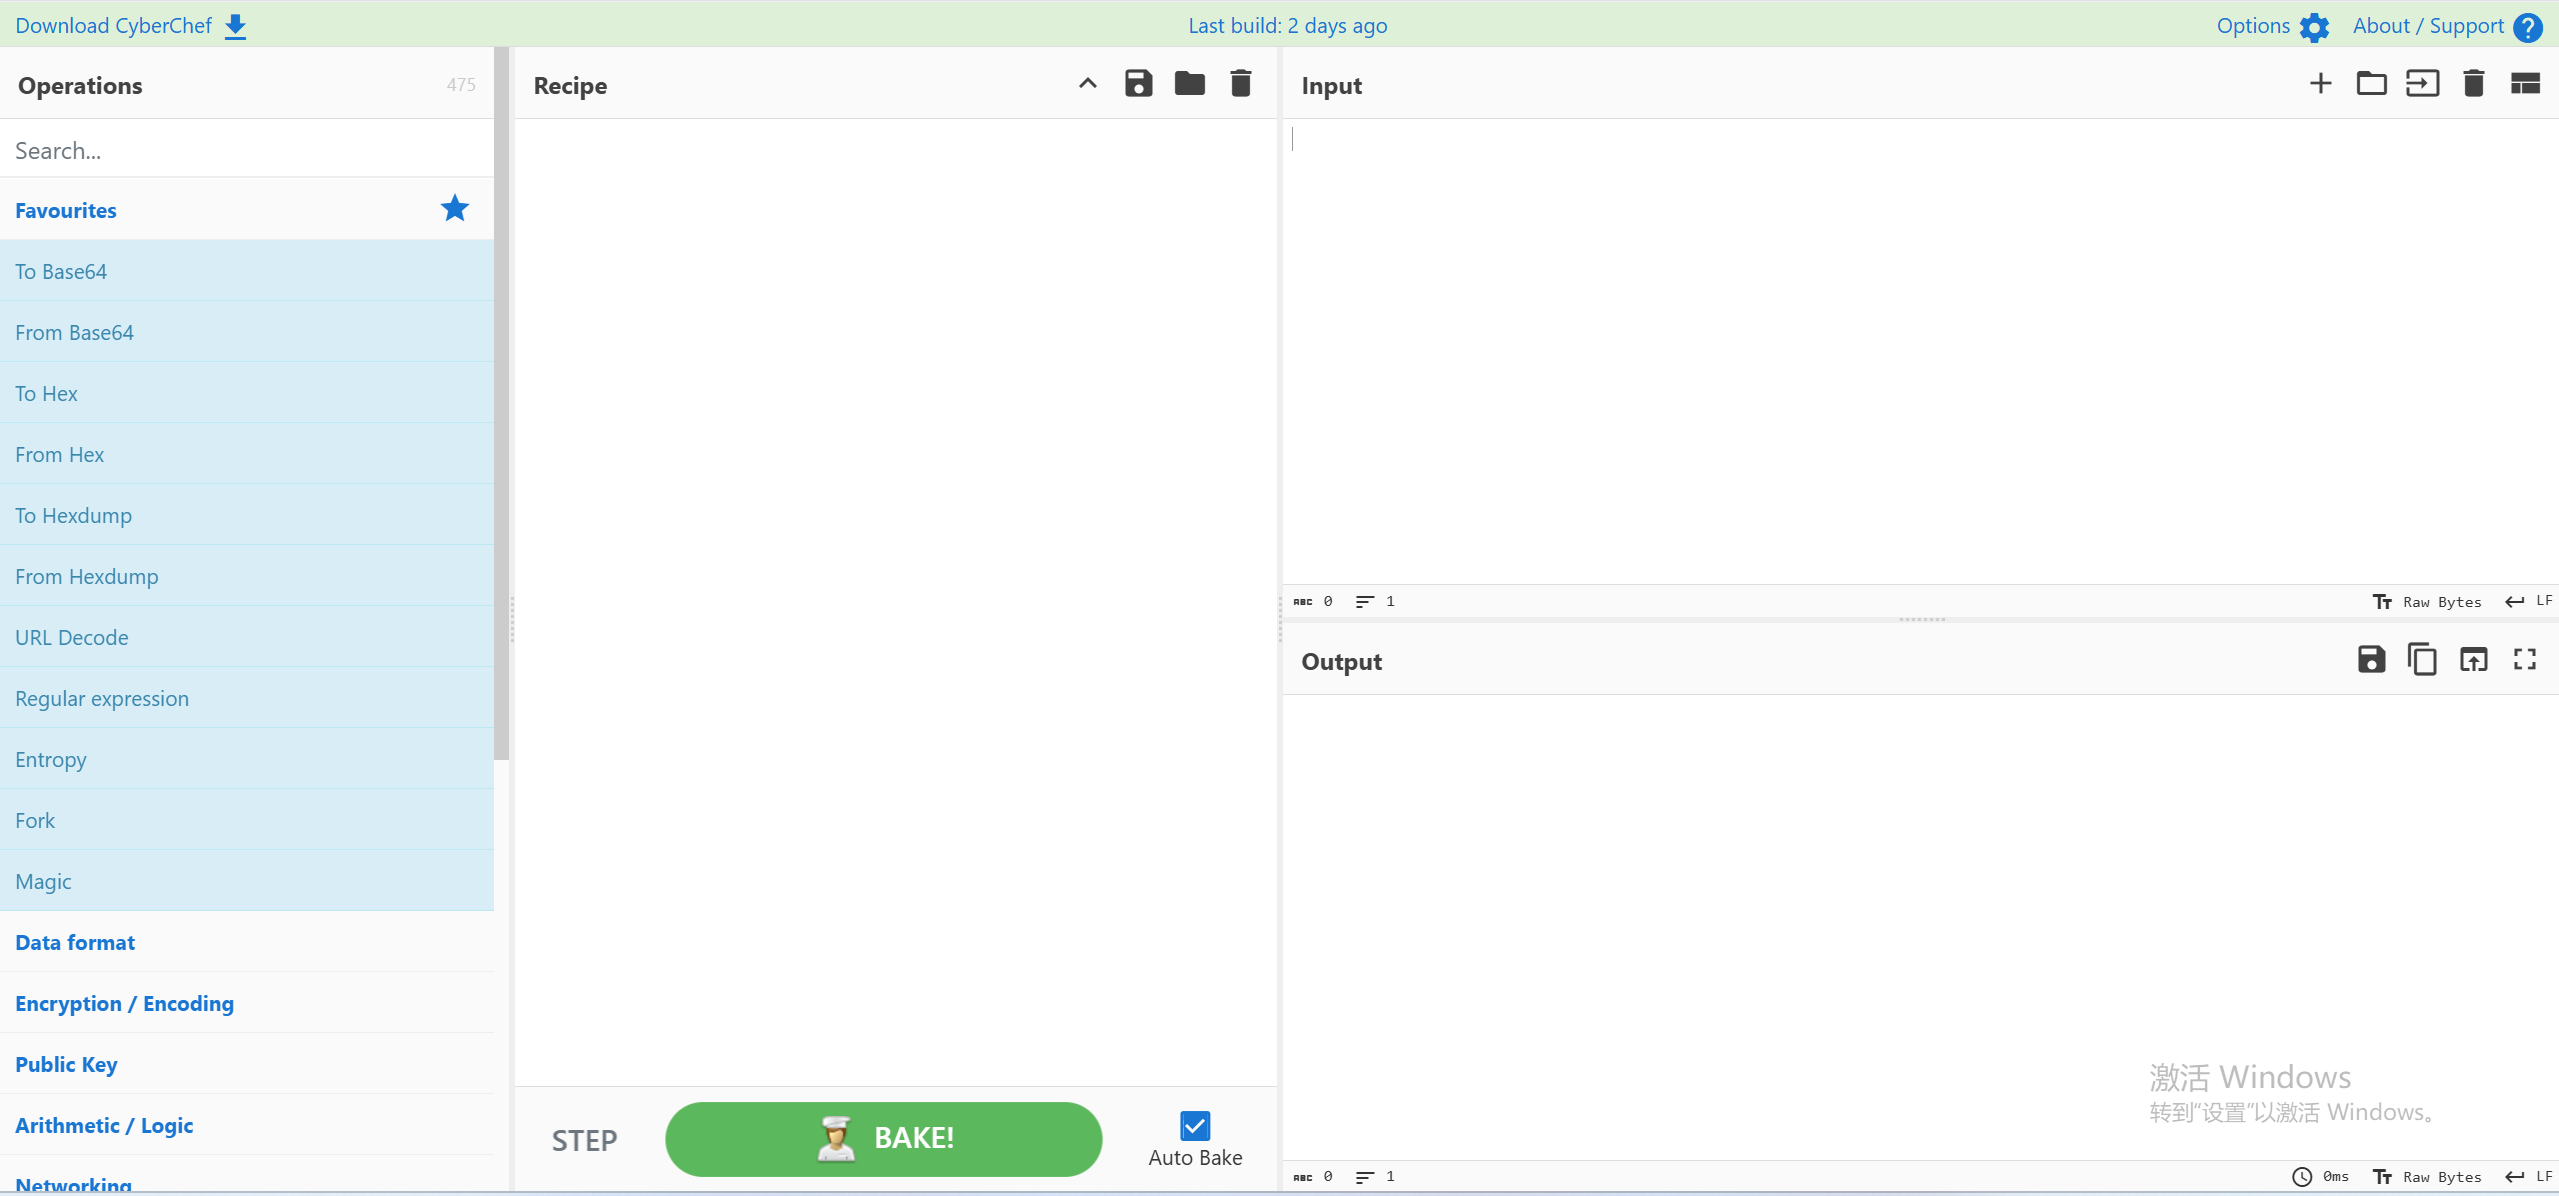
\includegraphics[width=0.9\textwidth]{4.1.png}
    \caption{CyberChef 工具界面与工作流程}
\end{figure}

工具使用流程：
\begin{enumerate}[leftmargin=*]
    \item \textbf{Input}：输入待处理数据
    \item \textbf{Operations}：选择需要的操作
    \item \textbf{Recipe}：组合多步处理操作
    \item \textbf{Output}：点击 BAKE! 获得结果
\end{enumerate}

\subsection{编码分析}
\subsubsection{常见编码方式}
CTF 中高频出现的编码类型：
\begin{itemize}[leftmargin=*]
    \item ASCII 编码
    \item Base64 / Base32 等 Base 系列编码
    \item 摩尔斯电码
    \item ROT 系列编码
    \item Unicode 编码（含连字、NFKC 标准化）
    \item URL 编码
\end{itemize}

参考资料：\url{https://ctf-wiki.org/misc/encode/computer/#base}

\subsubsection{编码载体与常见场景}
\begin{itemize}[leftmargin=*]
    \item \textbf{载体形式}：flag 通常以编码字符串形式隐藏
    \item \textbf{签到题}：直接给出多层嵌套编码
    \item \textbf{隐藏题}：编码内容藏于流量、图片等文件中，需先提取再解码
\end{itemize}

\subsubsection{Base 系列编码特征}
\textbf{Base64 编码特征：}
\begin{itemize}[leftmargin=*]
    \item 字符集：A–Z、a–z、0–9、+、/
    \item 结尾可能有填充符 =
\end{itemize}

\textbf{Base32 编码特征：}
\begin{itemize}[leftmargin=*]
    \item 字符集：A–Z、2–7
    \item 仅大写字母与数字，无 +/
    \item 结尾可能有填充符 =
\end{itemize}

\subsection{PyJail 沙箱逃逸例题：Truncate}
\subsubsection{题目源码与分析}
\begin{lstlisting}[language=Python]
#!/usr/bin/python3 -S
flag = open("flag.txt", "r").read().strip()
eval(input("")[:8])
\end{lstlisting}

\paragraph{代码解析}
\begin{itemize}[leftmargin=*]
    \item \texttt{-S}：禁用 site 模块，不影响本题核心逻辑
    \item 读取 flag.txt 内容存入变量 \texttt{flag}
    \item 获取用户输入，仅保留前 8 个字符，使用 \texttt{eval()} 执行
\end{itemize}

\paragraph{限制与目标}
\begin{itemize}[leftmargin=*]
    \item \textbf{限制}：输入长度最多 8 个字符
    \item \textbf{目标}：执行代码并泄露 \texttt{flag}
    \item \textbf{难点}：\texttt{print(flag)} 长度为 9，超出限制
\end{itemize}

\subsubsection{解题核心：Unicode 连字与 NFKC 标准化}
Python 在执行 \texttt{eval()} 前，会自动对字符串进行 NFKC 标准化。
部分 Unicode 连字字符会被展开为多个普通字符：
\begin{itemize}[leftmargin=*]
    \item \texttt{U+FB01} → \texttt{fi}
    \item \texttt{U+FB03} → \texttt{ffi}
    \item \texttt{U+FB00} → \texttt{ff}
\end{itemize}

利用该特性，可以实现\textbf{1 个字符输入 → 展开为多个字符}，从而突破长度限制。

\subsubsection{Payload 构造}
构造 Payload：
\[
\texttt{U+FB01 (flag)}
\]
经过 NFKC 标准化后变为：
\[
\texttt{int(flag)}
\]
长度仅 6 个字符，符合 8 字符限制，可成功执行并输出 flag。

\subsubsection{环境连接与执行}
\begin{itemize}[leftmargin=*]
    \item 环境：SEEDUbuntu 虚拟机
    \item 连接命令：\texttt{nc <IP> <Port>}
    \item 输入 Payload：\texttt{int(flag)} 获取 flag
\end{itemize}

\subsection{隐写术（Steganography）}
\label{subsec:misc_steganography_full}

\subsubsection{隐写术概述}
隐写术是将秘密信息隐藏在图片、音频、视频、文本、压缩包等载体中，实现隐蔽传输的技术，是 CTF Misc 中的核心考点。

\paragraph{CTF 中隐写术的常见特点}
\begin{itemize}[leftmargin=*]
    \item 题目多以文件附件形式给出，文件可能无后缀，需先识别文件类型
    \item 隐写术常与混淆、编码、密码学相结合，需多层分析才能提取 flag
\end{itemize}

\paragraph{常见载体}
\begin{itemize}[leftmargin=*]
    \item 图片（PNG、BMP）
    \item 音频（WAV、MP3）
    \item 文本（零宽字符隐写）
    \item 压缩包（伪加密、文件合并）
\end{itemize}

\subsubsection{文件识别基础}
\paragraph{文件识别方法}
\begin{itemize}[leftmargin=*]
    \item \textbf{后缀名识别}：通过文件后缀初步判断类型（不可靠，可伪造）
    \item \textbf{工具识别}：使用 \texttt{file} 命令（Linux）、\texttt{010 Editor} 等工具分析
    \item \textbf{文件头识别}：通过文件开头的魔数（Magic Number）精准识别文件类型（最可靠）
\end{itemize}

\paragraph{常见文件头对照表}
\begin{table}[htbp]
    \centering
    \caption{CTF 常见文件类型与对应文件头}
    \begin{tabular}{ll}
        \toprule
        文件类型 & 文件头（十六进制） \\
        \midrule
        JPEG (jpg) & FFD8FFE1 \\
        PNG (png) & 89504E47 \\
        GIF (gif) & 47494638 \\
        TIFF (tif) & 49492A00 \\
        Windows Bitmap (bmp) & 424DC001 \\
        ZIP Archive (zip) & 504B0304 \\
        RAR Archive (rar) & 52617221 \\
        Adobe Photoshop (psd) & 38425053 \\
        Rich Text Format (rtf) & 7B5C727466 \\
        XML (xml) & 3C3F786D6C \\
        HTML (html) & 68746D6C3E \\
        Adobe Acrobat (pdf) & 255044462D312E \\
        Wave (wav) & 57415645 \\
        pcap (pcap) & 4D3C2B1A \\
        \bottomrule
    \end{tabular}
\end{table}

\paragraph{文件操作常用工具}
\begin{itemize}[leftmargin=*]
    \item \textbf{判断文件类型}：\texttt{file}（Linux 命令）
    \item \textbf{查看/修改文件}：\texttt{WinHex}、\texttt{010 Editor}、\texttt{notepad++}、\texttt{Hex Editor}
    \item \textbf{分离文件}：\texttt{binwalk}、\texttt{foremost}、\texttt{dd}
    \item \textbf{文件检测/处理}：\texttt{Stegsolve}、\texttt{Pillow}
    \item \textbf{文件合并}：\texttt{cat}（Linux）、\texttt{copy}（Windows）
\end{itemize}

\subsubsection{图像隐写（LSB 隐写详解）}
\paragraph{LSB 隐写核心原理}
LSB（Least Significant Bit，最低有效位）是一种常见的信息隐藏方法。
图像像素一般由 RGB 三原色组成，每一种颜色占 8 位（\texttt{0x00~0xFF}，即 256 种颜色），而人的肉眼能区分的只有其中一小部分。

LSB 隐写就是修改 RGB 颜色分量中最低的二进制位：
\begin{itemize}[leftmargin=*]
    \item 仅修改像素中最低的 1 bit，肉眼完全无法区分前后变化
    \item 每个像素可携带 3 bit 信息（RGB 三通道各 1 bit）
    \item 不影响图片正常显示，同时隐藏秘密信息（通常为 \texttt{flag{xxx}} 格式）
\end{itemize}

\paragraph{StegSolve 实操步骤（图像隐写例题）}
\begin{enumerate}[leftmargin=*]
    \item 打开 StegSolve，加载目标图片
    \item 点击 \texttt{Analyse} → \texttt{Data Extract}
    \item 位平面设置：仅勾选 \textbf{Red 0、Green 0、Blue 0}（最低有效位）
    \item 字节序设置：选择 \texttt{LSB First}，\texttt{Bit Order} 选择 \texttt{RGB}
    \item 点击 \texttt{Preview} 查看隐藏数据，提取 flag 相关内容
\end{enumerate}

\subsubsection{音频隐写（摩斯码隐写详解）}
\paragraph{音频隐写核心原理}
音频隐写利用人耳对声音的不敏感特性，将秘密信息（如摩斯码）隐藏在音频文件中，通过分析音频波形提取信息。

\paragraph{工具：Audacity 实操步骤}
\begin{enumerate}[leftmargin=*]
    \item 打开 Audacity，加载音频文件 \texttt{secret.wav}
    \item 观察音频波形，识别有节奏的滴答声，对应摩斯码的点（·）和划（-）
    \item 提取摩斯码序列
    \item 使用在线摩斯码转换工具解码，得到 flag
\end{enumerate}

\paragraph{自动音频摩斯密码解码工具（无需看波形、无需听）}
\begin{itemize}[leftmargin=*]
    \item 在线音频摩斯自动解码：\url{https://morsecode.world/international/decoder/audio-decoder-adaptive.html}
    \item 功能：直接上传音频文件，自动识别摩斯密码并输出明文
    \item 适用场景：CTF 音频隐写（滴答声类型摩斯密码）
\end{itemize}

\paragraph{摩斯码隐写核心考点}
\begin{itemize}[leftmargin=*]
    \item 摩斯码基础：点（·）、划（-）、间隔（字符间隔/单词间隔）
    \item 音频波形分析：通过波形长短区分点和划
    \item 在线解码工具：快速将摩斯码转换为明文 flag
\end{itemize}

\subsubsection{文本隐写}
文本隐写利用不可见字符实现信息隐藏，典型为\textbf{零宽字符隐写}，将秘密信息编码进 Unicode 零宽字符中并嵌入普通文本，肉眼无法察觉。

\paragraph{常见零宽字符}
\begin{itemize}[leftmargin=*]
    \item 零宽空格（U+200B）
    \item 零宽连接符（U+200D）
    \item 零宽非连接符（U+200C）
\end{itemize}

\paragraph{分析工具与步骤}
\begin{itemize}[leftmargin=*]
    \item Sublime Text / VSCode：显示不可见字符，提取零宽字符序列
    \item 330k 官方零宽隐写工具：\url{http://330k.github.io/misc_tools/unicode_steganography.html}
    \item 备用在线工具：\url{https://www.mzy0.com/ctftools/zerowidth1/}
\end{itemize}

\paragraph{标准解题流程}
\begin{enumerate}[leftmargin=*]
    \item 将含隐写的文本粘贴至 330k 零宽字符隐写工具
    \item 点击 Decode 按钮直接提取隐藏信息
    \item 对解码结果进行整理，得到最终 flag
\end{enumerate}

\subsubsection{隐写术通用解题思路}
\begin{enumerate}[leftmargin=*]
    \item \textbf{文件类型识别}：用 \texttt{file}/\texttt{010 Editor} 识别载体，补全后缀
    \item \textbf{载体针对性分析}：
    \begin{itemize}[leftmargin=*]
        \item 图片：StegSolve 位平面与 LSB 提取
        \item 音频：Audacity 波形分析与摩斯码提取
        \item 文本：零宽字符提取与解码
        \item 压缩包：binwalk 提取并逐层解压
    \end{itemize}
    \item \textbf{编码/密码学处理}：对提取的信息进行解码、解密
    \item \textbf{按正则构造 flag 并提交}
\end{enumerate}

\subsection{隐写术常用工具汇总}
\begin{table}[htbp]
    \centering
    \caption{隐写术全载体常用工具清单}
    \begin{tabular}{ll}
        \toprule
        工具名称 & 工具用途 \\
        \midrule
        StegSolve / StegOnline & 图片位平面分析、LSB 提取、PNG 块分析 \\
        Audacity & 音频处理、摩斯码提取与分析 \\
        010 Editor & 16 进制编辑、文件头识别 \\
        Sublime Text & 零宽字符查看 \\
        330k Unicode Steganography & 零宽字符文本隐写解密 \\
        CyberChef & 编码解码、LSB 提取 \\
        binwalk & 隐藏文件提取 \\
        7-Zip / WinRAR & 压缩包解压 \\
        \bottomrule
    \end{tabular}
\end{table}

\subsection{网络安全竞赛通用工具清单}
\begin{table}[htbp]
    \centering
    \caption{网络安全竞赛全题型常用工具}
    \begin{tabular}{ll}
        \toprule
        工具类别 & 代表工具 \\
        \midrule
        渗透测试 & Burp Suite、Nmap、Metasploit \\
        逆向分析 & IDA Pro、Ghidra、x64dbg \\
        密码学 & CyberChef、John the Ripper、Hashcat \\
        取证分析 & Wireshark、Volatility、Foremost \\
        \bottomrule
    \end{tabular}
\end{table}

\subsection{参考文献}
\begin{enumerate}[leftmargin=*]
    \item 《CTF那些事儿》，李舟军，机械工业出版社，2023
    \item 《CTF特训营：技术详解、解题方法与竞赛技巧》，FlappPig战队著，机械工业出版社，2022
    \item 《CTF竞赛权威指南（Pwn篇）》，杨超，电子工业出版社，2020
    \item 《白帽子Web安全》，吴翰清，电子工业出版社，2021
    \item 《CTF安全竞赛入门》，张镇等，清华大学出版社，2020
    \item Unicode 标准与规范化形式：\url{https://unicode.org/reports/tr15/}
    \item Python eval 与 Unicode 标准化：\url{https://docs.python.org/3/reference/lexical_analysis.html#unicode-normalization}
    \item 摩斯码在线转换工具：\url{http://mosi.fjnews.com/}
    \item 音频摩斯密码自动解码工具：\url{https://morsecode.world/international/decoder/audio-decoder-adaptive.html}
    \item 零宽字符隐写工具：\url{http://330k.github.io/misc_tools/unicode_steganography.html}
\end{enumerate}
\section{Web 安全}
\label{sec:web}

\subsection{Web 安全概述}
Web 安全是 CTF 竞赛中最核心、最常见的题型，主要考察参赛人员对 HTTP 协议、Web 应用漏洞原理、漏洞利用工具、代码审计及渗透测试思路的掌握程度，覆盖前后端全栈安全知识。

\subsubsection{Web 核心学习参考}
\begin{itemize}[leftmargin=*]
    \item CTF Wiki Web 安全：\url{https://ctf-wiki.org/web/}
    \item Burp Suite 实战指南：\url{https://blog.csdn.net/qq_35544379/article/details/76696106}
    \item SQL 注入从入门到精通：\url{https://blog.csdn.net/phppppppppp/article/details/124968358}
    \item Hackbar 工具使用教程：\url{https://blog.csdn.net/weixin_49769267/article/details/131501614}
\end{itemize}

\subsubsection{Web 核心考察方向}
Web 题目涉及知识面广泛，核心考点主要包括：
\begin{itemize}[leftmargin=*]
    \item SQL 注入漏洞与利用
    \item 文件上传漏洞与解析绕过
    \item PHP 特性与代码执行绕过
    \item XSS 跨站脚本攻击
    \item CSRF 跨站请求伪造
    \item SSRF 服务器端请求伪造
    \item 反序列化漏洞
    \item HTTP 协议与请求包构造
\end{itemize}

\newpage
% --------------------- 常用工具
\subsection{Web 常用工具介绍}
\begin{table}[htbp]
    \centering
    \caption{Web 题型常用工具清单}
    \begin{tabular}{ll}
        \toprule
        工具名称 & 工具用途 \\
        \midrule
        Burp Suite & Web 渗透集成平台，代理、重放、爆破、扫描 \\
        Sqlmap & 自动化 SQL 注入检测与利用工具 \\
        Hackbar & Firefox 插件，快速构造 HTTP 请求 \\
        Dirsearch & Web 目录扫描、隐藏路径爆破 \\
        蚁剑/冰蝎/Weevely & 网站后门管理、文件管理、命令执行 \\
        Nmap & 端口扫描、服务探测 \\
        Wireshark & HTTP/HTTPS 流量抓包与分析 \\
        \bottomrule
    \end{tabular}
\end{table}

\subsubsection{Kali Linux 渗透测试系统}
Kali Linux 是基于 Debian 的 Linux 发行版，专为渗透测试、数字取证设计，预装大量 Web 安全工具，是 CTF Web 题目的标准实验环境。
\begin{itemize}[leftmargin=*]
    \item 官网：\url{https://www.kali.org/}
    \item 核心工具：Burp Suite、Sqlmap、Nmap、Wireshark 等
\end{itemize}

\newpage
% --------------------- 核心工具详解
\subsection{核心工具详解}

\subsubsection{Hackbar 工具}
Hackbar 是 Firefox 浏览器插件，用于快速编辑、发送 HTTP 请求，支持编码解码、加密、参数修改，是 Web 入门必备工具。

\begin{itemize}[leftmargin=*]
    \item 加载 URL、快速修改 GET/POST 参数
    \item 支持 URL、Base64、16 进制编码解码
    \item 支持 MD5、SHA1、SHA256 哈希计算
    \item 一键发送请求，查看响应结果
\end{itemize}

\subsubsection{Burp Suite 工具}
Burp Suite 是 Web 安全最核心工具，提供完整渗透测试工具链：
\begin{itemize}[leftmargin=*]
    \item \textbf{Proxy}：HTTP/HTTPS 代理，拦截修改请求
    \item \textbf{Repeater}：手动重放 HTTP 请求
    \item \textbf{Intruder}：暴力破解、Fuzz 测试
    \item \textbf{Decoder}：编码解码工具箱
\end{itemize}

\subsubsection{SQLmap 工具}
SQLmap 是自动化 SQL 注入工具，可自动检测、利用注入漏洞，获取数据库权限、数据。

常用命令：
\begin{itemize}[leftmargin=*]
    \item 探测注入点：\texttt{sqlmap -u "url"}
    \item 枚举所有数据库：\texttt{--dbs}
    \item 查看表名：\texttt{-D 库名 --tables}
    \item 脱库数据：\texttt{--dump}
\end{itemize}

\newpage
% --------------------- HTTP 协议基础
\subsection{HTTP 请求协议基础}

\subsubsection{GET 请求}
\begin{itemize}[leftmargin=*]
    \item 用于从服务器获取数据
    \item 参数直接拼接在 URL 中
    \item 长度受限、参数可见
\end{itemize}

\subsubsection{POST 请求}
\begin{itemize}[leftmargin=*]
    \item 用于向服务器提交数据
    \item 参数放在请求体中
    \item 长度无限制、更安全
\end{itemize}

\subsubsection{HTTP 常见请求头}
\begin{itemize}[leftmargin=*]
    \item \textbf{Host}：目标主机地址
    \item \textbf{User-Agent}：客户端标识
    \item \textbf{Cookie}：用户身份凭证
    \item \textbf{Referer}：请求来源页面
    \item \textbf{X-Forwarded-For}：客户端真实 IP
\end{itemize}

\newpage
% --------------------- HTTP 请求示例
\subsection{HTTP 请求示例}

\subsubsection{GET 请求示例}
\begin{verbatim}
GET /index.html HTTP/1.1
Host: www.test.com
User-Agent: Mozilla/5.0
Accept: */*
Connection: close
\end{verbatim}

\subsubsection{POST 请求示例}
\begin{verbatim}
POST /login HTTP/1.1
Host: www.test.com
Content-Type: application/x-www-form-urlencoded
Content-Length: 20

username=admin&password=123
\end{verbatim}

\newpage
% --------------------- Hackbar 实验
\subsection{Hackbar 使用实验}

\subsubsection{实验目的}
\begin{itemize}[leftmargin=*]
    \item 掌握 GET/POST 请求区别
    \item 能够使用 Hackbar 构造、修改、发送 HTTP 请求
    \item 理解 HTTP 请求头作用并能手动修改
    \item 完成基础 Web 题目测试
\end{itemize}

\subsubsection{实验步骤}
\begin{enumerate}[leftmargin=*]
    \item 安装 Firefox 与 Hackbar 插件
    \item 加载目标 URL，熟悉工具面板
    \item 构造 GET 请求，修改参数并发送
    \item 构造 POST 请求，填写请求体数据
    \item 修改 Referer、X-Forwarded-For 等请求头
    \item 观察服务器响应并记录结果
\end{enumerate}

\subsubsection{实验要求}
\begin{itemize}[leftmargin=*]
    \item 独立完成 HTTP 请求构造
    \item 熟练使用编码解码功能
    \item 提交完整实验记录与测试截图
\end{itemize}

\newpage
% --------------------- 通用解题思路
\subsection{Web 安全通用解题思路}
\begin{enumerate}[leftmargin=*]
    \item \textbf{信息收集}：目录扫描、端口扫描、查看页面源码
    \item \textbf{抓包分析}：使用 Burp Suite 抓取 HTTP 请求
    \item \textbf{漏洞判断}：识别 SQL 注入、文件上传、XSS 等漏洞
    \item \textbf{工具利用}：使用 SQLmap、Hackbar 等完成利用
    \item \textbf{权限提升}：获取网站权限、读取 flag
    \item \textbf{提交 flag}
\end{enumerate}

\newpage
% --------------------- 参考文献
\subsection{参考文献}
\begin{enumerate}[leftmargin=*]
    \item CTF Wiki Web 安全官方文档：\url{https://ctf-wiki.org/web/}
    \item 《白帽子讲 Web 安全》，吴翰清，电子工业出版社
    \item 《CTF 特训营：技术详解、解题方法与竞赛技巧》
    \item Burp Suite 官方文档：\url{https://portswigger.net/burp/documentation}
    \item SQLmap 官方使用手册：\url{https://sqlmap.org/}
    \item HTTP 协议官方标准：\url{https://www.w3.org/Protocols/rfc2616/rfc2616.html}
\end{enumerate}
\end{document}